\documentclass{ximera}  
\title{Flowcharts}  
\usepackage{tikz}
\usetikzlibrary{shapes.geometric, arrows}
\tikzstyle{startstop} = [rectangle, rounded corners, minimum width=3cm, minimum height=1cm,text centered, draw=black, fill=red!30]
\tikzstyle{io} = [trapezium, trapezium left angle=70, trapezium right angle=110, minimum width=3cm, minimum height=1cm, text centered, draw=black, fill=blue!30]
\tikzstyle{process} = [rectangle, minimum width=3cm, minimum height=1cm, text centered, draw=black, fill=orange!30]
\tikzstyle{decision} = [diamond, minimum width=3cm, minimum height=1cm, text centered, draw=black, fill=green!30]
\tikzstyle{arrow} = [thick,->,>=stealth]
\begin{document}  
\begin{abstract}  
We introduce flowcharts as a way to organize a procedure designed to solve a particular problem.
\end{abstract}  
\maketitle

An algorithm is a fixed set of instructions that can be followed to solve a problem. Algorithms take in a set of inputs from a predifined set, perform a series of clearly defined computations, and produce an output meant to solve a particular problem. While it mmay take a while for an algorithm to produce an answer (say, if the size of the input is large), it should always be the case that the solution to the problem is found in a finite amount of time.

There are several ways to specify an algorithm. For now we will represent our algorithms using a special type of diagram known as a flowchart. As we gain more experience we will be able to transition to other methods for expressing algorithms. We begin with flowcharts because they are a relatively intuitive to use and because you probably have some prior experience with them.

Here, for example, are two different algorithms for accomplishing the same task. 

\begin{figure}[!ht]
	\centering
	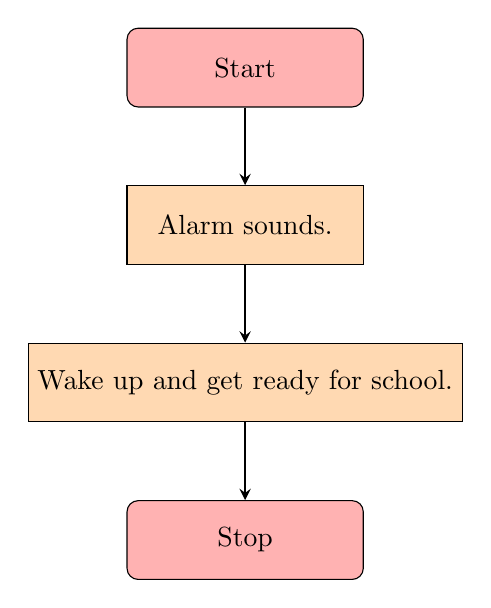
\begin{tikzpicture}
		\node (start) [startstop] {Start};
		\node (alarm) [process, below of = start, yshift = -1cm] {Alarm sounds.};
		\node (wake) [process, below of = alarm, yshift = -1cm] {Wake up and get ready for school.};
		\node (stop) [startstop, below of = wake, yshift = -1cm] {Stop};
		\draw [arrow] (start) -- (alarm);
		\draw [arrow] (alarm) -- (wake);
		\draw [arrow] (wake) -- (stop);
	\end{tikzpicture}
	\caption{An example of an algorithm for your morning routine.}
\end{figure}

\begin{figure}[!ht]
	\centering
	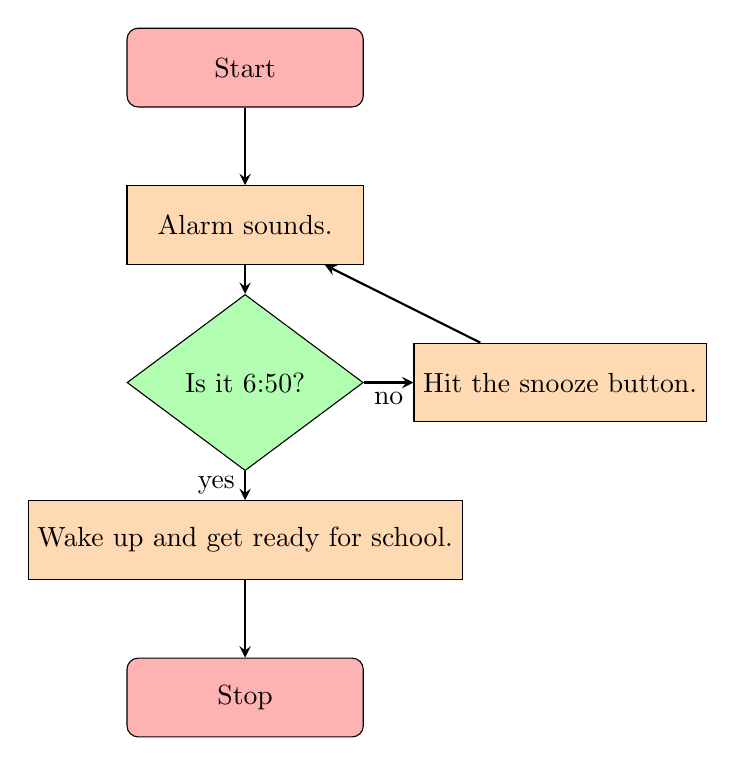
\begin{tikzpicture}
		\node (start) [startstop] {Start};
		\node (alarm) [process, below of = start, yshift = -1cm] {Alarm sounds.};
		\node (check) [decision, below of = alarm, yshift = -1cm] {Is it 6:50?};
		\node (wake) [process, below of = check, yshift = -1cm] {Wake up and get ready for school.};
		\node (snooze) [process, right of = check, xshift = 3cm] {Hit the snooze button.};
		\node (stop) [startstop, below of = wake, yshift = -1cm] {Stop};
		\draw [arrow] (start) -- (alarm);
		\draw [arrow] (alarm) -- (check);
		\draw [arrow] (check) -- node[anchor=north] {no} (snooze);
		\draw [arrow] (check) -- node[anchor=east] {yes} (wake);
		\draw [arrow] (snooze) -- (alarm);
		\draw [arrow] (wake) -- (stop);
	\end{tikzpicture}
	\caption{Another example of an algorithm for your morning routine.}
\end{figure}

\end{document}
